\documentclass[class=report, crop=false, 12pt,a4paper]{standalone}
\usepackage{enumitem}
\usepackage{multicol}
\usepackage{etoolbox}
\AtBeginEnvironment{quote}{\singlespacing\small}
\usepackage{setspace}
\onehalfspacing
\usepackage{graphicx}
\usepackage{float}
\usepackage{amsmath}
\usepackage{amssymb}
\usepackage{siunitx}
\sisetup{detect-all}
\begin{document}
\section{Refrigeration cycles}
It is well known that heat flows in the direction of decreasing temperature i.e from a high temperature region to a low temperature. But the reverse process (i.e. heat transfer from low to high temperature) cannot occur by itself. This requires a special device called a refrigerator. Another device which transfers heat from a low to high temperature is a heat pump. Heat pump and refrigerator cycles are very similar. The difference is in their objectives. The most frequently used refrigeration cycle is the vapour-compression refrigeration cycle. The refrigerant is vaporised and condensed alternately and is compressed in the vapour phase. 

Another well known cycle is the gas refrigeration cycle, in which the refrigerant remains in the gaseous phase throughout. Refrigerators are cyclic devices and the working fluids used in the refrigeration cycles are called refrigerants.
\begin{figure}
  \centering
  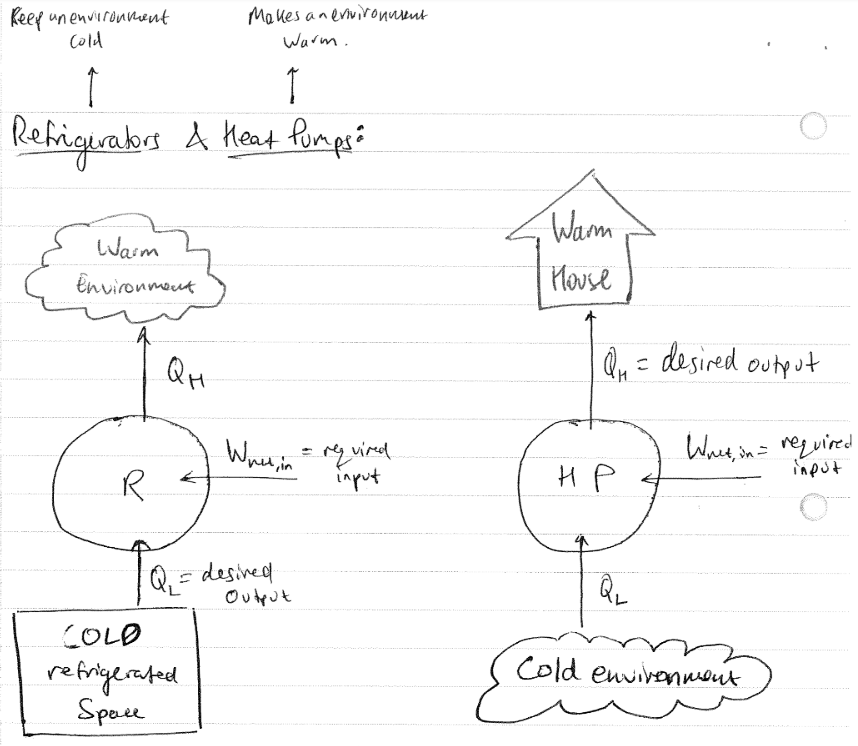
\includegraphics[width = 0.8\textwidth]{../img/RefigerationCycles}
  \caption{Diagrams for refrigeration cycles.}
\end{figure}
The performance of refrigerators and heat pumps is expressed in terms of coefficient of performance (COP).
\begin{align}
  COP_R &= \frac{\textrm{Desired output}}{\textrm{Required input}} = \frac{Q_L}{W_{net, \ in}} \ \textrm{(can be greater than 1)}\\
  COP_{HP} &= \frac{\textrm{Desired output}}{\textrm{Required input}} = \frac{Q_H}{W_{net, \ in}} > 1\\
  COP_{HP} &= COP_R +1
\end{align}
Thus, since $COP_R$ is a positive quantity $\therefore COP_{HP} >1$.
\subsection{The reversed Carnot cycle}
This was touched upon in \ref{reversecarnot} on page \pageref{reversecarnot}. Recall that the Carnot cycle is a totally reversible cycle which consists of two reversible isothermal processes and two isentropic processes. It has the maximum efficiency for a given temperature limit. Since it is a reversible cycle, all four processes can be reversed. This will reverse the direction of heat and work interactions, therefore producing a refrigeration cycle. A refrigerator or heat pump that runs on this cycle is called a Carnot refrigerator or a Carnot heat pump.

The cycle consists of: 
\begin{itemize}[noitemsep]
  \item Process 1-2: isothermal heat transfer from cold medium to refrigerant in an evaporator.
  \item Process 2-3: isentropic (reversible adiabatic) compression in a compressor. 
  \item Process 3-4: isothermal heat rejection (condenser).
  \item Process 4-1: isentropic expansion (turbine).
\end{itemize}
\subsection{Components of a reversed Carnot cycle}
\begin{figure}
  \centering
  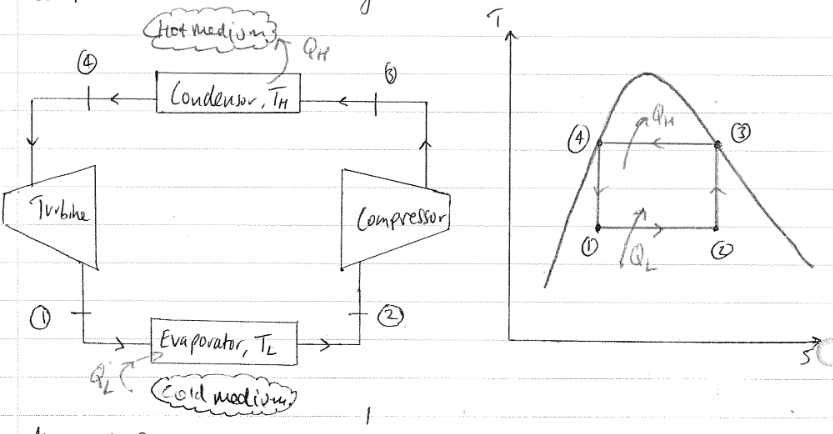
\includegraphics[width = 0.7\textwidth]{../img/ComponentsReversedCarnot}
  \caption{Components of a reversed Carnot cycle and Ts diagram.}
\end{figure}
Also:
\begin{equation}
  COP_{R, \ Carnot} = \frac{1}{\frac{T_H}{T_L} -1}
\end{equation}
and
\begin{equation}
  COP_{HP, \ Carnot} = \frac{1}{1 - \frac{T_L}{T_H}}
\end{equation}
Both COP's increase as the difference between the two temperatures decreases. The reversed Carnot cycle is the \emph{most efficient} refrigeration cycle operating between two specified temperature levels. However, the reversed Carnot cycle is not a suitable model for a refrigeration cycle as:
\begin{itemize}[noitemsep]
  \item Process 2-3 requires a compressor that can handle two phases.
  \item Process 4-1 involves the expansion of high-moisture-content refrigeration in a turbine
\end{itemize}
\subsection{The ideal vapour compression refrigeration cycle}
Many of the impracticalities associated with the reversed Carnot cycle can be eliminated by vaporising the refrigerant completely before it is compressed and by replacing the turbine with a throttling device such as an expansion valve or capillary tube. The ideal vapour-compression refrigeration cycle consists of four processes:
\begin{itemize}[noitemsep]
  \item Process 1-2: isentropic compression in a compressor.
  \item Process 2-3: isobaric heat rejection in a condenser.
  \item Process 3-4: throttling in an expansion device.
  \item Process 4-1: isobaric heat absorption in an evaporator.
\end{itemize}
\subsection{Components of an ideal vapour compression refrigerator}
\begin{figure}
  \centering
  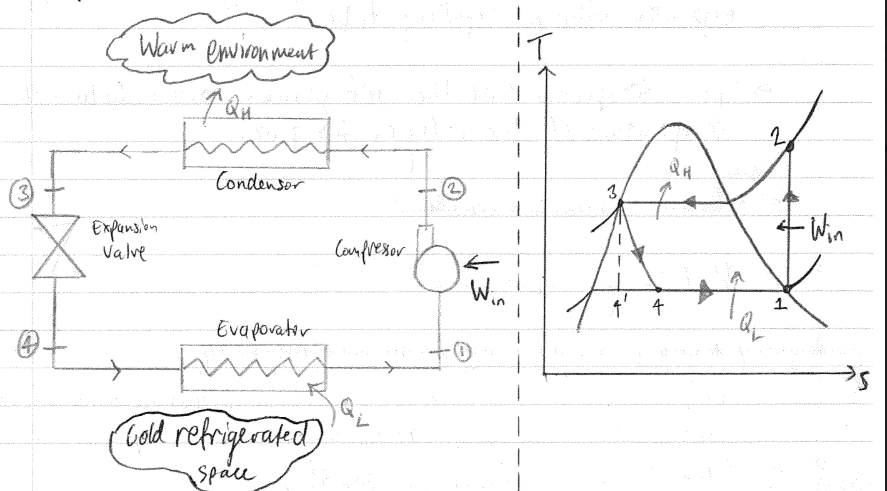
\includegraphics[width = 0.7\textwidth]{../img/ComponentsAndTsIdealVCR}
  \caption{Components of an ideal vapour compression refrigerator and Ts diagram.}
\end{figure}
\subsection{Qualitative description of the ideal vapour compression cycle}
\subsubsection{Process 1-2}
Enters compressor as a saturated vapour. Compressed isentropically to the condenser pressure. Temperature of refrigerant increases (higher than surroundings).
\subsubsection{Process 2-3}
Enters the condenser as a superheated vapour. Heat is rejected to the surroundings. Refrigerant leaves as a saturated liquid at stage 3. Still, the temperature of the refrigerant is higher than the surroundings. 
\subsubsection{Process 3-4}
The saturated liquid refrigerant at state 3 is throttled to the evaporator pressure by passing it through an expansion valve or capillary tube. The temperature of the refrigerant drops below the temperature of the refrigerated space. (Note that unlike the ideal cycles discussed before , the ideal vapour compression cycle is not an internally reversible cycle, since it involves an irreversible throttling process. If the throttling device is replaced by an isentropic turbine, the refrigerant would reach state 4!)
\subsubsection{Process 4-1}
Enters as state 4, low quality saturated mixture. Completely evaporates by absorbing heat from the refrigerated space. Leaves the condenser as saturated vapour and cycle restarts.

Remember that the area under the process of a Ts diagram represents the heat transfer for internally reversible processes. The area under process 4-1 is the heat absorbed by the refrigerant. The area under process 2-3 is the heat rejected in the condenser. Tip: for each increase in $T_H$ or decrease in $T_L$, in \si{\celsius}/\si{\kelvin}, the COP improves.
\subsection{Ph diagram}
Another diagram frequently used in the analysis of vapour compression refrigeration cycles is the Ph diagram. A Ph diagram is made respectively for a specified refrigerant. it can, of course, not be used for a another refrigerant. A Ph diagram has a lot of thin lines, whose names and natures are important. 
\begin{figure}
  \centering
  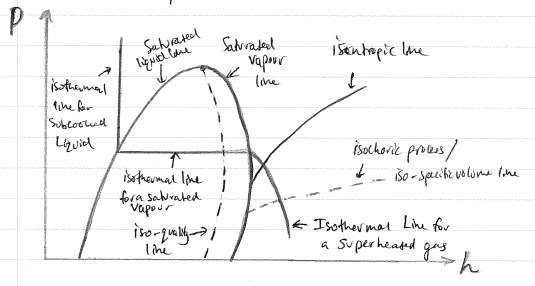
\includegraphics[width = 0.7\textwidth]{../img/PhDiagram}
  \caption{A Ph diagram.}
\end{figure}
\subsection{Ph diagram for the ideal vapour compression refrigeration cycle}
\begin{figure}
  \centering
  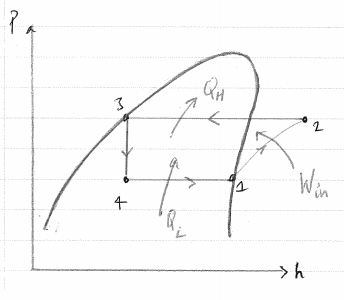
\includegraphics[width = 0.7 \textwidth]{../img/PhDiagram2}
  \caption{Ph diagram for the ideal vapour compression refrigeration cycle.}
\end{figure}
\subsection{Energy analysis of the ideal vapour compression refrigeration cycle}
All four components are steady flow devices. Neglect kinetic and potential energy changes as they are usually small relative to the work and heat transfer terms. Applying SFEE per unit mass:
\begin{align}
  \dot{Q}_{in} + \dot{W}_{in} + \dot{m} h_1 &= \dot{Q}_{out} + \dot{W}_{out} + \dot{m} h_2\\
  q_{in} + w_{in} + h_1 &= q_{out} + w_{out} + h_2
\end{align}
\subsubsection{Compressor: Process 1-2}
\begin{gather}
  q = 0, \ w_{out} = 0\\
  w_{in} = h_2 - h_1 \ \si{\kilo\joule\per\kg} \textrm{ where } h_1 = h_{g@P_1}
\end{gather}
\subsubsection{Condenser: Process 2-3}
\begin{gather}
  q_{in} = 0, \ w = 0 \\
  q_{out} = h_2 - h_3\\
  q_H = h_2 - h_3
\end{gather}
\subsubsection{Expansion valve: Process 3-4 (throttling process)}
\begin{gather}
  q = 0, \ w = 0\\
  h_3 = h_4 \textrm{ (isentropic process)}
\end{gather}
Remember that process 2-3 is an isobaric process. Hence:
\begin{equation}
  P_2 = P_3
\end{equation}
Thus, since $h_3 = h_{f@P_3} \rightarrow h_3 = h_{f@P_2}$. Also, process 3-4 is isenthalpic.
\begin{equation}
  \therefore h_3 = h_4 \rightarrow h_4 = \left( h_f \right)_{P_2} \label{refrigeq1}
\end{equation}
But $h_4 = \left( h_f \right)_{P_H} + x_4 \left(h_{fg} \right)_{P_H}$
\begin{equation}
  (P_1 = P_4) \rightarrow h_4 = \left( h_f \right)_{P_1} + x_4 \left(h_{fg} \right)_{P_1}
  \label{refrigeq2}
\end{equation}
Equation \ref{refrigeq1} = Equation \ref{refrigeq2}
\begin{align}
  h_4 = \left( h_f \right)_{P_2} &= \left( h_f \right)_{P_1} + x_4 \left(h_{fg} \right)_{P_1}\\
  \therefore x_4 &= \frac{\left( h_f \right)_{P_2} - \left( h_f \right)_{P_1}}{\left( h_{fg} \right)_{P_1}}
\end{align}
Where $x_4$ is the quality of the refrigerant at the inlet of the evaporator.
\subsubsection{Evaporator: Process 4-1}
\begin{gather}
  w = 0, \ q_{out} = 0\\
  q_{in} = h_1 - h_4\\
  q_L = h_1 - h_4
\end{gather}
Where $q_L = h_1 - h_4$ represents the refrigeration effect.
\subsection{Coefficient of performance}
From the definition of heat pumps and refrigerators:
\begin{equation}
  COP_R = \frac{q_L}{w_{net, \ in}} = \frac{h_1 - h_4}{h_2 - h_1}
\end{equation}
And
\begin{equation}
  COP_{HP} = \frac{q_H}{w_{net, \ in}} = \frac{h_2 - h_3}{h_2 - h_1}
\end{equation}
If $\dot{m}$ is the mass flow of refrigerant in \si{\kg\per\second} then,
\begin{align}
  \dot{Q}_L &= \dot{m}q_L = \dot{m} (h_1 - h_4) \ \si{\kg\per\second}\\
  &= \dot{m} (h_1 - h_4) \times 3600 \ \si{\kg\per\hour}
\end{align}
One tonne of refrigeration: the rate of heat removal equivalent to the heat required for melting one tonne of ice in one day. If the total latent heat of fusion is 335 \si{\kilo\joule\per\kg} = $h_{fg}$ then one tonne of refrigeration is:
\begin{equation}
  \frac{336 \times 10^{3}}{24} = 14000 \ \si{\kilo\joule\per\hour}
\end{equation}
Therefore, the cooling capacity of the refrigeration plant (rate of heat removal from the refrigerated space) is:
\begin{equation}
  \textrm{cooling capacity of the refrigeration plant} = \frac{\dot{m}(h_1 - h_4) \times 3600}{14000}
\end{equation}
Similarly,
\begin{gather}
  \textrm{heat removed from the condenser} = \dot{m} q_H = \dot{m} (h_2 - h_3) = \dot{Q}_H\\
  \textrm{power at compressor} = \dot{W}_{in} = m\dot{w}_{in} = \dot{m} (h_2 - h_1)\\
  \textrm{volume of gas handled by the compressor, flow rate} = \dot{V} = \dot{m}v
\end{gather}
\end{document}